\documentclass[preprint, prb]{revtex4-1}
\usepackage{amsmath}
\usepackage{amssymb}
\usepackage{graphicx}
\usepackage{enumitem}
\usepackage{bm}
\usepackage[font={footnotesize}]{caption}
\usepackage{todonotes}
\usepackage{comment}
\graphicspath{{./}{./images/}}
\definecolor{darkblue}{rgb}{0.1,0.2,0.6} \definecolor{darkred}{rgb}{0.8,0.1,0.2}
\usepackage[colorlinks,citecolor=darkblue,linkcolor=darkred,urlcolor=darkblue]{hyperref}
\usepackage[all]{hypcap}

\renewcommand{\vec}[1]{\boldsymbol{\mathbf{#1}}}

\newcommand{\cf}{\textit{cf.} } 
\newcommand{\ie}{\textit{i.e.} } 
\newcommand{\eg}{\textit{e.g.} }
\newcommand{\vs}{\textit{vs.} } 
\newcommand{\etal}{\textit{et al.} }
\newcommand{\etc}{\textit{etc.} }

\begin{document}

\title{Bipartite Fidelity and Loschmidt Echo of Bosonic Conformal Interface}
 
\author{Tianci Zhou}
\email{tzhou13@illinois.edu}
\affiliation{University of Illinois, Department of Physics, 1110 W. Green St. Urbana, IL 61801 USA}

\author{Mao Lin}
\email{maolin2@illinois.edu}
\affiliation{University of Illinois, Department of Physics, 1110 W. Green St. Urbana, IL 61801 USA}

\date{\today}

\begin{abstract}
\end{abstract}

\maketitle

\section{Introduction}


% quantum impurity problem,  boundary critical phenomena, Anderson orthogonality catastrophe
In (one-dimensional) quantum critical systems, the presence of the physical boundary and isolated impurity weakly break the conformal symmetry of the system. Simply put, the scattering on the interface relates the otherwise independent modes and therefore demonstrates novel boundary critical phenomena\cite{cardy_boundary_2004}. Operators close to the boundary are interpreted as boundary condition changing (bcc) operators\cite{oshikawa_boundary_1997,affleck_boundary_1997} in the boundary conformal field theory (CFT). Their correlation functions can exhibit different critical exponents from the bulk counterparts\cite{cardy_conformal_1984}. One example is the ``Anderson orthogonality catastrophe", where the core hole creates a potential that acts as an impurity to the conduction band. The X-ray absorption rate will then have a power singularity of boundary exponent\cite{affleck_boundary_1997} at the resonance frequency. There are numerous impurity problems of this kind that have been studied in the last few decades, such as the magnetic impurity in spin chain\cite{eggert_magnetic_1992}, boundary and impurity effects in Luttinger liquid\cite{fabrizio_interacting_1995}, entanglement of the defects\cite{peschel_entanglement_2005, igloi_entanglement_2009,calabrese_entanglement_2012} \etc

% non-equilibrium dynamics, particle mediate the two parts, Cardy cut-and-join protocol, Vassur majarana
Recently, more attention has been paid to the non-equilibrium dynamics of the quantum impurity\cite{hegde_quench_2015,francica_local_2016,lupo_transient_2016,lee_spatiotemporal_2016,chung_memory_2016,sacramento_edge_2016,vasseur_expansion_2015,mazza_overlap_2016}. The ``cut-and-join" quench protocol is a popular framework for studying the spreading of the influence from the localized impurity (or boundary) across the system. As shown in the left panel of Fig.~\ref{fig:cut-and-join}, the system consists of two critical chains A and B, which were prepared in the ground states. They will be joined at $t = 0$ and evolve. Various quantities can be used to detect the information in the quench process. For instance, Ref.~\onlinecite{calabrese_entanglement_2007, calabrese_quantum_2016} find a logarithmic increase of entanglement entropy in subsystem $A$, when both $A$ and $B$ are identical critical systems. The authors ascribe such increase to the proliferation and propagation of quasi-particle excitations emitted at the joint. Ref.~\onlinecite{vasseur_universal_2014} takes A to be a normal lead and B to be a topological superconductor in the topological phase. In this model, the Majorana zero mode acts as a bcc and its conformal dimension appears in the exponent of the power law decay for the Loschmidt echo.

\begin{figure}[h]
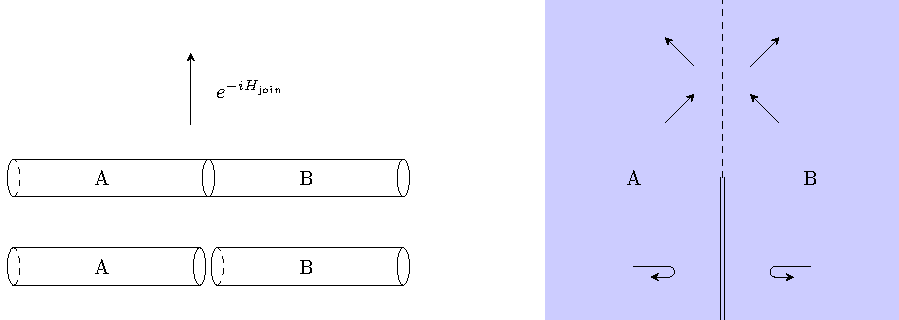
\includegraphics[width=1\columnwidth]{fig_cut_and_join.pdf}
\caption{Cut-and-join quench protocol. Left panel: Prepare the ground states of two separated chains and join them at $t = 0$, then time evolve with the whole chain Hamiltonian. Right panel: Spacetime diagram of the cut and join protocol. The solid line represents the boundaries of the two disconnected chains. It is totally reflective for the incident particles on both sides. The dashed line is the world line of the junction, which we will call interface. It could either be totally transparent or partially permeable, depending the types of theories of A and B.}
\label{fig:cut-and-join}
\end{figure}

% All of these are the same CFTs. we consider different CFTs, the mediating particle or primary field will be different, from the S matrix point of view.
In the path integral language, the ``cut-and-join" protocol corresponds to a spacetime diagram as shown in the right panel of Fig.~\ref{fig:cut-and-join}. The separating ground states prepared before $t = 0$ are joined to form a new type of interface between them. Before the quench, the slit represents boundaries that are completely reflective to the injecting particles. The joining turns on the transmission from one side to the other. In the entanglement entropy and Loschmidt echo examples cited above\cite{calabrese_entanglement_2007, calabrese_quantum_2016, vasseur_universal_2014}, the two sides of the CFTs are the same (chiral fermion CFT in the case of Ref.~\onlinecite{vasseur_universal_2014}) and the boundary becomes totally transparent after the joining. 

In this paper, we generalize these ideas and consider connecting two different CFTs in the ``cut-and-join" protocol. The interface produced will interpolate between the total reflective and complete transparent ones. As discussed in Ref.~\onlinecite{bachas_permeable_2002}, such interface can be realized as a domain wall between two free compact boson theories with different compactification radii. Entanglement properties for non-compact free boson/free fermion lattices have been numerically and analytically studied\cite{peschel_exact_2012,sakai_entanglement_2008}. In these models, there is a parameter $\lambda$ that is directly related to the transmission coefficient. In the case of compact boson $\lambda$ is controlled by the ratio of the compactification radii, whereas it is controlled by the ratio of masses in the case of free lattice boson. We expect it to be tunable in a realistic experimental setting.

% fidelity and Loschmidt echo are quantities that extract boundary critical exponents, may reveal the nature of the mediating particle 
We compute the Loschmidt echo to extract information in the dynamics of the quench process. The Loschmidt echo is the (square of) overlap of the wavefunctions before the quench and the wavefunction evolved for some time $t$. It decays with a power law $t^{- \alpha}$for the lack of length scale in the $t \rightarrow \infty$ limit. The decay exponent $\alpha$ has been calculated for various geometries and combinations of the normal boundary conditions of the same CFTs in \onlinecite{stephan_logarithmic_2013,stephan_local_2011}. We extend the analysis to the aforementioned parametric interface of (possibly) different CFTs. We will see that there are two categories of the scattering matrices $S(\theta)$ of the interfaces, whose scattering angle parameter $\theta$ is determined by the transition coefficients. Our analytic and numerical results show that $\alpha$ has a quadratic dependence on the change of $\theta$ if the prior and post quench boundary conditions are in the same type of $S$, while remains $\frac{1}{4}$ otherwise. The finite size fidelity calculation further supports these results. 

The rest of the paper is organized as follows. In Sec.~\ref{sec:bosonic_conformal_interface}, we introduce the general formalism for permeable conformal interface and its lattice realization. In Sec.~\ref{sec:analytic_numerics}, we analytically evaluate the free energy associated with fidelity and Loschmidt echo, and present the numerical results for comparison. We discuss our results and related experimental works in Sec.~\ref{sec:disc}. Finally, we conclude in Sec.~\ref{sec:conclusion}. 

This paper includes several appendices for technical details. In App.~\ref{app:lambda_12}, we present the detailed calculation of the free energy for the above-mentioned interfaces. In App.~\ref{app:gnd_dn_lambda}, we illustrate an alternative approach with one setup as an example. In App.~\ref{app:F_correction}, we point out two corrections to the free energy, which are complementary to the argument made in the main text. Up to this point, we work exclusively with the oscillator modes of the free bosons. In App.~\ref{app:compact_diff_boson}, it is shown that the winding modes of compactified bosons will \emph{not} contribute to the free energy at the leading order. Therefore, the results remain valid in the physical situation of connecting two compactified bosons of different radii. In App.~\ref{app:pf_of_id}, we prove one identity that will be used repeatedly in the analytical evaluation. We derive the scale invariant interface for free bosonic lattice in App.~\ref{app:interface_free_boson}. The details of numerical simulation are presented in App.~\ref{app:comp_fid_echo}.  

%%% Local Variables:
%%% TeX-master: "bCFT_paper"
%%% TeX-PDF-mode: t
%%% End:


\section{Bosonic Conformal Interface}
\subsection{General Formulation}
% M, S
% special case
\subsection{Physical Realization: Connecting Bosons of Different Compactification Radii}
% free boson + compact
\subsection{A Free Boson Lattice Model}
% cite Calabrese, introduce the model
% lattice model S matrix

\section{Bipartite Fidelity and Loschmidt Echo}
\subsection{Definition}
% definition
% general discussion

\section{Analytic and Numerical Results}
\subsection{Fidelity}
% analytic: conformal transformation
% numerical comparison
\subsection{Loschmidt Echo}
% analytic: conformal transformation
% numerical comparison

\section{Discussion}

% connecting Luttinger liquid(quantum wire) using votage to control the boundary condition. X-ray edge singularity. examples include Taylor santo's topological phases. Hope to have experimental setup. 
There are already numerous theoretical and experimental work on the boundary conditions of Luttinger liquid\cite{schmeltzer_zero_1999,anfuso_luttinger_2003,voit_bounded_2000,fabrizio_interacting_1995,egger_applying_1998}, which is the universal compact boson theory of the (Bosonized) one-dimensional electron gas\cite{giamarchi_quantum_2015}. For example, gate voltage \cite{egger_applying_1998} may be used to twist the left and right modes of the boson to create a boundary condition interpolating between the normal open and fixed boundary conditions. The interface studied in this paper is a generalization which (in the folding picture) twist the two independent Bosons (two left modes plus two right modes) on the two sides. 

\begin{acknowledgments}
\todo[inline]{Thomas Faulkner, Xueda Wen, Shinsei Ryu, Romain Vasseur}
    TZ is supported by the National Science Foundation under grant number NSF-DMR-1306011.
    This work made use of the Illinois Campus Cluster, a computing resource that is operated by the
    Illinois Campus Cluster Program (ICCP) in conjunction with the National Center for
    Supercomputing Applications (NCSA) and which is supported by funds from the University of
    Illinois at Urbana-Champaign.
\end{acknowledgments}

\appendix
\section{Corrections to the Free Energy}
% two corrections:
% 1. staircase geometry
% 2. contribution from the boundary: cite Cardy 

\section{Numerical Computation of Bipartite Fidelity and Loschmidt Echo}
% basis transformation, Bogoliubov state, overlap(master theorem)
% Peschel_EE.pdf
\label{app:comp_fid_echo}

In this appendix, we provide technical details about the numerical calculation of the bipartite fidelity and Loschmidt echo.  Our strategy takes advantage of the symplectic structure of the bosonic Bogoliubov transformation and explicitly construct the "BCS" like ground state. With slight modification\cite{blaizot_quantum_1986}, one can work out its fermionic version and apply to quadratic fermion models in Ref.~\onlinecite{vasseur_universal_2014,stephan_local_2011}.

During the course of derivation in this and other appendices, we will repeatedly use the combinatorial identity called McMahon Master theorem
\begin{equation}
\label{eq:bosonic_McMahon}
\langle0|\exp\left\{\frac{1}{2}b_iX_{ij}b_j\right\}\exp\left\{\frac{1}{2}b^\dagger_iY_{ij}b^\dagger_j\right\}|0\rangle=\text{det}^{-\frac{1}{2}}(1-XY),
\end{equation}
for symmetric matrix $X$ and $Y$ and set of independent bosonic creation operators $b_i^{\dagger}$. One can prove it for (simultaneously) diagonalizable matrices and then claim its legitimacy for its combinatorial nature. 

\subsection{Boson Bogoliubov transformation}
\label{app_sub:boson_BdG}
We consider the following quadratic bosonic Hamiltonian
\begin{equation}
\begin{aligned}
\label{eq:quadratic_boson_H}
\hat{H} &= \frac{1}{2} (\vec{b}^{\dagger}, -\vec{b}) M 
\begin{pmatrix}
\vec{b}\\
\vec{b}^{\dagger} 
\end{pmatrix},  \qquad 
M = 
\begin{bmatrix}
A & -B^* \\
B & -A^* \\
\end{bmatrix},
\end{aligned}
\end{equation}
where ${\bf b}\equiv(b_{1},...,b_{n})^T$ is a vector of bosonic annihilation operators. The matrix $M$ consists of a $n\times n$ Hermitian block $A$ which plays the role of single particle Hamiltonian in the fermionic case and symmetric block $B$ of the pairing interaction. 

We want to do a Bogoliubov transformation, which uses a $2n \times 2n$ matrix $S$ to define a diagonal basis 
\begin{equation}\begin{aligned}
\label{eq:def_a}
({\bf a} , {\bf a}^\dagger)\equiv({\bf b} , {\bf b}^\dagger)S
\end{aligned}\end{equation}
of the Hamiltonian. The transformation is canonical, meaning that it preserves the commutation relation 
\begin{equation}
\begin{aligned}
\label{eq:preserve_commutator}
J&\equiv\begin{bmatrix}
0 & \mathbb{I}\\
-\mathbb{I} & 0
\end{bmatrix}
=[
\begin{pmatrix}
{\bf a} \\
{\bf a}^\dagger
\end{pmatrix},
\begin{pmatrix}
{\bf a} & {\bf a}^\dagger
\end{pmatrix}]
=S^T[
\begin{pmatrix}
{\bf b} \\
{\bf b}^\dagger
\end{pmatrix},
\begin{pmatrix}
{\bf b} & {\bf b}^\dagger
\end{pmatrix}]S \\
&=S^T JS,
\end{aligned}
\end{equation}
where we have used the compact notation of the sort $([\vec{b}, \vec{b}^{\dagger}])_{ij} =  [b_i, b_j^\dagger]$ to denote the commutator matrix. The appearance of $J$ makes the symplectic nature of the problem manifest and we find $S$ is in the symplectic group ${\rm Sp}( 2n, \mathbb{C} ) $\cite{blaizot_quantum_1986,fulton_representation_2004}. Furthermore, the requirement that $a^\dagger$ is a complex conjugation of $a$ leads to the block structure of $S$
\begin{equation}
\label{eq:block_S}
S=
\begin{bmatrix}
u & v^*\\
v & u^*
\end{bmatrix}.
\end{equation}
And the blocks are constrained by the symplectic property
\begin{eqnarray}
  u^\dagger u-v^\dagger v&=\mathbb{I},\label{eq:constraint_1}\\
  u^T u-v^T v&=0\label{eq:constraint_2}.  
\end{eqnarray}
With these conditions, the Hamiltonian in basis $a$ becomes (the use of $({\bf b}^\dagger , -{\bf b})$ rather than $({\bf b}^\dagger , {\bf b})$ can be appreciated in this step)
\begin{equation}
H = \frac{1}{2} ( a^{\dagger}, -a )  (S^{\top} M (S^{\top})^{-1} )
\begin{pmatrix}
a\\
a^{\dagger} 
\end{pmatrix}.
\end{equation}
Quiet unusually, the diagonalization is performed by the symplectic group element.

To proceed, we introduce the real basis 
\begin{equation}\begin{aligned}
\label{eq:real_basis}
\begin{pmatrix}
{\bf b}\\
{\bf b}^\dagger
\end{pmatrix}
=C\begin{pmatrix}
\phi\\
\pi
\end{pmatrix}
=\frac{1}{\sqrt{2}}\begin{bmatrix}
1 & i \\
1 & -i
\end{bmatrix}\begin{pmatrix}
\phi\\
\pi
\end{pmatrix},
\end{aligned}\end{equation}
in which the Hamiltonian reads
\begin{equation}\begin{aligned}
\hat{H}
&=\frac{1}{2}
\begin{pmatrix}
\phi & \pi
\end{pmatrix}
\begin{bmatrix}
\text{Re}(A-B^*) & -\text{Im}(A)+\text{Im}(B)\\
\text{Im}(A)+\text{Im}(B)& \text{Re}(A+B) \\
\end{bmatrix}
\begin{pmatrix}
\phi\\
\pi
\end{pmatrix} \\
&=\frac{1}{2}
\begin{pmatrix}
\phi & \pi
\end{pmatrix}
\mathcal{M}
\begin{pmatrix}
\phi\\
\pi
\end{pmatrix}.
\end{aligned}\end{equation}
It is not hard to check that $\mathcal{M}$ is real and symmetric. 

The general solution of the diagonalization problem is hard\cite{arnold_mathematical_2010}, however the positive definite $\mathcal{M}$ (and hence $M$) case can be solved by Williamson's theorem\cite{arnold_mathematical_2010,xiao_theory_2009,pirandola_correlation_2009,gosson_symplectic_2006}, which states the existence, uniqueness (up to reordering of eigenvalues) and explicit construction of the matrix $\mathcal{S}\in {\rm Sp}(2n \mathbb{R}) $ such that 
\begin{equation}\begin{aligned}
\mathcal{M}=\mathcal{S}
\begin{bmatrix}
\, d \, & \\
 & \, d\, \\
\end{bmatrix}
\mathcal{S}^T,
\end{aligned}\end{equation}
where the diagonal matrix $d$ are positive eigenvalues of $iJ\mathcal{M}$. After some algebra, we have
\begin{equation}\begin{aligned}
\label{eq:diagonalization_M}
M=J(C^{-1})^T\mathcal{S}C^TJ^{-1}
\begin{bmatrix}
d\\
&-d
\end{bmatrix}
C\mathcal{S}^TC^{-1}.
\end{aligned}\end{equation}
One can show that,
\begin{equation*}\begin{aligned}
S\equiv C\mathcal{S}^TC^{-1}
\end{aligned}\end{equation*}
is the required symplectic matrix in the complex basis. 

We will not elaborate on Williamson's theorem and its proof (see proofs in Ref.~\onlinecite{xiao_theory_2009,pirandola_correlation_2009,gosson_symplectic_2006} and also a recent application in entanglement entropy context\cite{coser_contour_2017}). Instead we will show in App.~\ref{app_sub:harmonic_chain} that for the problem of harmonic chain we are interested in, the diagonalization can be easily done without using the general recipe in the Williamson theorem. 


\subsection{Groundstate in $b$ Basis}

Suppose we have obtained the required matrix $S$, the ground state will be the vacuum of the annihilation operators defined in Eq.~\eqref{eq:def_a} and in $b$ basis it satisfies
\begin{equation}\begin{aligned}
\label{eq:a_vacuum_condition}
(b_iu_{ij}+b_i^\dagger v_{ij})|0\rangle_{{\bf a}}=0.
\end{aligned}\end{equation}
If the matrix $u$ is invertible, then we can introduce a matrix $T=vu^{-1}$ to rewrite Eq.~\eqref{eq:a_vacuum_condition} as
\begin{equation}\begin{aligned}
(b_i+b_j^\dagger T_{ji})|0\rangle_{{\bf a}}=0. 
\end{aligned}\end{equation}
The constraint Eq.~\eqref{eq:constraint_2} on the blocks of $u$ and $v$ (followed by the symplectic constraint of $S$) implies that $T$ is a symmetric matrix. With the observation of 
\begin{equation}\begin{aligned}
\exp\left\{-\frac{1}{2}b_j^\dagger T_{jk}b_k^\dagger\right\}b_i\exp\left\{\frac{1}{2}b_j^\dagger T_{jk}b_k^\dagger\right\}=b_i+T_{ij}b^\dagger_j,
\end{aligned}\end{equation}
we solve the groundstate
\begin{equation}\begin{aligned}
\label{eq:boson_BCS_gnd}
|0\rangle_{{\bf a}}&=\text{det}^{\frac{1}{4}}(1-T^\dagger T)\exp\left\{-\frac{1}{2}b_j^\dagger T_{jk}b_k^\dagger\right\}|0\rangle_{\bf b},\\
\end{aligned}\end{equation}
where the normalization is given by the McMahon Master theorem Eq.~\eqref{eq:bosonic_McMahon}. Apply constraint in Eq.~\eqref{eq:constraint_1}, it simplifies to the top left corner of the symplectic matrix
\begin{equation}
\text{det}^{\frac{1}{4}}(1-T^\dagger T) =|\text{det}(u)|^{-\frac{1}{2}}.
\end{equation}

Eq.~\eqref{eq:boson_BCS_gnd} takes a similar form as the superconducting ground state, with the pairing wavefunction $T_{ij}$ determined by the Bogoliubov transformation. In the next section, we will see that the normalization factor gives the fidelity and Loschmidt echo.

\subsection{Boson fidelity} 
\label{app_sub:boson_fidelity}

Fidelity is defined as the (squared) overlap of groundstates of two different bosonic Hamiltonians. 

We start with a quadratic bosonic Hamiltonian $\hat{H}_0$ in ${\bf b}$ basis, as in Eq.~\eqref{eq:quadratic_boson_H}. From the discussion in App.~\ref{app_sub:boson_BdG}, we are able to diagonalize it in ${\bf a}$ basis for positive definite $M$. At $t=0$, the Hamiltonian becomes $\hat{H}_1$, which is still written in ${\bf b}$ basis, but is diagonalized in a new basis ${\bf c}$. The corresponding Bogoliubov transformations read
\begin{equation}\begin{aligned}
\label{eq:two_BdG}
({\bf b} , {\bf b}^\dagger)S_0=({\bf a} , {\bf a}^\dagger),\quad
({\bf b} , {\bf b}^\dagger)S_1=({\bf c} , {\bf c}^\dagger),
\end{aligned}\end{equation}
and so
\begin{equation}\begin{aligned}
\label{eq:S0invS}
({\bf a} , {\bf a}^\dagger)=({\bf c} , {\bf c}^\dagger)\left(S_0^{-1}S_1\right)^{-1}.
\end{aligned}\end{equation}
One realizes that Eq.~\eqref{eq:S0invS} is another Bogoliubov transformation and so the corresponding matrix has the block structure
\begin{equation}
S_1^{-1}S_0=\begin{bmatrix}
u_1 & v_1^*\\
v_1 & u_1^*
\end{bmatrix}.
\end{equation}
Thus $|0\rangle_{\bf c}$ is related to the $|0\rangle_{{\bf a}}$ in the same way as in Eq.~\eqref{eq:boson_BCS_gnd}. Their overlap is therefore given by the normalization factor
\begin{equation}\begin{aligned}
|{}_{\bf a}\langle0|0\rangle_{\bf c}|^2=\frac{\Big|{}_{\bf a}\langle 0 | \exp( -\frac{1}{2} a_j^{\dagger} T^{jk} a_k^{\dagger} )|0   \rangle_{\bf a} \Big|^2}{|\text{det}(u_1)|} = \frac{1}{|\text{det}(u_1)|}.
\end{aligned}\end{equation}

\subsection{Boson Loschmidt echo}
\label{app_sub:boson_Loschmidt_echo}

The Loschmidt echo is defined as the (squared) overlap of the evolved state
\begin{equation}\begin{aligned}
|0\rangle_{{\bf a}(t)}\equiv e^{-i\hat{H}_1t}|0\rangle_{\bf a},
\end{aligned}\end{equation}
with $|0\rangle_{\bf a}$ the ground state of the Hamiltonian $\hat{H}_0$ before the quench. We introduce a dynamical basis
\begin{equation}\begin{aligned}
a_i(t)&=e^{-i\hat{H}_1t}a_ie^{i\hat{H}_1t},
\end{aligned}\end{equation}
which annihilate the evolved state at time $t$: $a_i(t)|0\rangle_{{\bf a}(t)}=0$. Upon using the diagonal basis $\hat{H}_1=\sum_iE_ic_i^\dagger c_i$, the Bogoliubov transformation at time $t$ can be represented as a chain of symplectic transformation
\begin{equation}\begin{aligned}
\label{eq:BdG_transformation_echo}
&({\bf a}(t),{\bf a}^\dagger(t))=e^{-iHt}
({\bf a} , {\bf a}^\dagger)e^{iHt} \\
=&({\bf a},{\bf a}^\dagger)S_0^{-1}S_1\text{diag}(e^{iEt},e^{-iEt})S_1^{-1}S_0.
\end{aligned}\end{equation}
It is evident that the evolved state $|0\rangle_{{\bf a}(t)}$ is related to the $|0\rangle_{{\bf a}}$ in the same way as in Eq.~\eqref{eq:boson_BCS_gnd}. The overlap, as we have seen in the fidelity case, is the normalization factor of the "BCS" ground state. It is related to the top left block of the Bogoliubov transformation in Eq.~\eqref{eq:BdG_transformation_echo},
\begin{equation}\begin{aligned}
\label{eq:echo_t}
\mathcal{L}(t)=|_{\bf a}\langle0|0\rangle_{{\bf a}(t)}|^2=|\text{det}(u_1^\dagger e^{iEt}u_1-v_1^\dagger e^{-iEt}v_1)|^{-1}.
\end{aligned}\end{equation}

\subsection{Harmonic chain} 
\label{app_sub:harmonic_chain}

In this subsection, we explicitly construct the matrix $\mathcal{S}$ for the case of harmonic chain introduced in Sec.~\ref{sec_sub:free_boson_lattice}. In the basis defined in Eq.~\eqref{eq:real_basis}, the Hamiltonian for 1D harmonic chain reads
\begin{equation}\begin{aligned}
\hat{H}
=\frac{1}{2}
\begin{pmatrix}
\phi & \pi
\end{pmatrix}
\mathcal{M}
\begin{pmatrix}
\phi\\
\pi
\end{pmatrix}
=\frac{1}{2}
\begin{pmatrix}
\phi & \pi
\end{pmatrix}
\begin{bmatrix}
\mathcal{V} \\
& {\mathbb{ I}}
\end{bmatrix}
\begin{pmatrix}
\phi\\
\pi
\end{pmatrix},
\end{aligned}\end{equation}
where $\mathcal{V}$ is real symmetric matrix that can be diagonalized as $\mathcal{V}=\mathcal{O}D^2\mathcal{O}^T$. The matrix $\mathcal{V}$ depends on the boundary condition, but positive definiteness is the only requirement here. 

The matrix $\mathcal{S}$ that diagonalize $\mathcal{M}$,
\begin{equation}
\begin{aligned}
\mathcal{M}=\mathcal{S}
\begin{bmatrix}
D \\ 
& D
\end{bmatrix}
\mathcal{S}^T
\end{aligned}
\end{equation}
is given by the following real symplectic matrix
\begin{equation}\begin{aligned}
\mathcal{S}\equiv
\begin{bmatrix}
\mathcal{O}D^{1/2} \\
& \mathcal{O}D^{-1/2}
\end{bmatrix}.
\end{aligned}\end{equation}


Thus the Hamiltonian is diagonalized as
\begin{equation}\begin{aligned}
M=S^{-1}
\begin{bmatrix}
D \\
& -D
\end{bmatrix}
S,
\end{aligned}\end{equation}
where the Bogoliubov transformation take the desired block form
\begin{equation}\begin{aligned}
S&=C\mathcal{S}C^{-1}
=\begin{bmatrix}
O(D^{1/2}+D^{-1/2}) & O(D^{1/2}-D^{-1/2}) \\
O(D^{1/2}-D^{-1/2}) & O(D^{1/2}+D^{-1/2}) 
\end{bmatrix}.
\end{aligned}\end{equation}


%%% Local Variables:
%%% TeX-master: "bCFT_paper"
%%% TeX-PDF-mode: t
%%% End:


\section{A Determinant Identity for the Boundary State Amplitude}
\label{app:pf_of_id}
% copy notes app. C
% flatex input: [pf_of_id.tex]

In this appendix, we provide more details for calculating the amplitude $Z_{ab}$ in Sec.{\bf\color{red}where}. We started to prove the following identity for a real symmetric matrix $M$
\begin{equation}
\label{eq:first_id_app_pf_of_id}
\exp\Big\{- \vec{b}^{\dagger} M \vec{b}  \Big\} \exp \Big\{ \vec{b}^{\dagger} R \bar{\vec{b}}^{\dagger}  \Big\}  = \exp \Big\{ \vec{b}^{\dagger} e^{-M}  R \bar{\vec{b}}^{\dagger}  \Big\} \exp\Big\{- \vec{b}^{\dagger} M \vec{b}  \Big\} 
\end{equation}
where ${\bf b}$ and $\bar{\bf b}$ are vectors of bosonic operators. As emphasized in the {\bf\color{red}main text}, the matrix notation, for example, $\vec{b}^{\dagger} R \bar{\vec{b}}^{\dagger}$ should really mean $\sum_{ij}b^\dagger_iR_{ij}\bar{b}_j^\dagger$ where the dagger does not transpose the vector.  

To prove Eq.~\eqref{eq:first_id_app_pf_of_id}, we first consider the special case where $R=\mathbb{I}$. We diagonalize $M = O^{T} \Lambda O $ and rotate the two sets of boson operators to the diagonal basis
\begin{equation}
  \vec{b}^{\dagger}  M \vec{b} = \vec{d}^{\dagger} \Lambda \vec{d}  \quad \vec{d} = O \vec{b} \quad \vec{\bar{d}}^\dagger = O^T \vec{\bar{b}}^\dagger
\end{equation}
where we understood $\vec{\bar{b}}^\dagger$ is a column vector and independent to $\vec{{b}}^\dagger$. Thus the whole expression can be written as
\begin{equation}
\begin{aligned}
  \exp&\Big\{- \vec{b}^{\dagger} M \vec{b}  \Big\} \exp \Big\{ \vec{b}^{\dagger} \bar{\vec{b}}^\dagger  \Big\}  =  
  \exp\Big\{- \vec{d}^{\dagger} \Lambda \vec{d}  \Big\} \exp \Big\{   \vec{d}^{\dagger} \bar{\vec{d}}^\dagger  \Big\} \\
& = \prod_i  \exp\Big\{- \lambda_i d_i^{\dagger} d_i  \Big\} \exp \Big\{  d_i^{\dagger} \bar{d}_i ^{\dagger}  \Big\}
\end{aligned}
\end{equation}
We recall for $ [X, Y] = sY $, 
\begin{equation}
  e^X e^{Y} = e^{\exp (s ) Y} e^{X}
\end{equation}
which is a solvable case of Baker-Campbell-Hausdorff formula. Upon taking $X = -\lambda_i d_i^{\dagger} d_i$, $Y = d_i^{\dagger} \bar{d}^{\dagger}_i$, we have
\begin{equation}
\label{eq:lambda_commutator}
[- \lambda_i d_i^{\dagger} d_i, d_i ^{\dagger} \bar{d}_i^{\dagger}] =  - \lambda_i  d_i ^{\dagger} \bar{d}_i^{\dagger} 
\end{equation}
and so $s = - \lambda_i$ for each $\lambda_i$. This enable us to commute those exponentials
\begin{equation}
\begin{aligned}
 \exp\Big\{- \vec{b}^{\dagger} M \vec{b}  \Big\} \exp \Big\{  \vec{b}^{\dagger} \bar{\vec{b}}^\dagger  \Big\}   &= \prod_i \exp \Big\{ e^{- \lambda_i }  d^{\dagger}_i \bar{d}^{\dagger}_i  \Big\}  \exp \Big\{-\lambda_i  d^{\dagger}_i d_i  \Big\} \\
 & = \exp \Big\{ \vec{b}^{\dagger} e^{-M}  \bar{\vec{b}}^\dagger  \Big\} \exp\Big\{- \vec{b}^{\dagger} M \vec{b}  \Big\} 
\end{aligned}
\end{equation}
For the general case where $R \neq\mathbb{I}$, we take $\vec{\bar{d}}^* = O^T R \vec{\bar{b}}^*$. This will not change the commutation relation of ${\bf d}$, and the role of $\bar{b}$ is decorative in Eq.~\eqref{eq:lambda_commutator}. Hence the rest of the proof follows the same way. \hfill$\blacksquare$

A direct consequence of Eq.~\eqref{eq:first_id_app_pf_of_id} is the following
\begin{equation}
\label{eq:second_id_in_app_pf_of_id}
Z_{ab} = \langle 0 | \exp\Big\{ \vec{b} R_a^* \vec{\bar{b}}\Big\} \exp\Big\{ - \vec{b}^{\dagger} M  \vec{b} \Big\}   \exp\Big\{  \vec{b}^{\dagger} R_b  \vec{\bar{b}}^{\dagger}\Big\}  |0  \rangle  = \frac{1}{\det( 1- R_a^{\dagger} e^{-M} R_b )} 
\end{equation}
where $|0\rangle$ is the vacuum for ${\bf b}$ and $\bar{\bf b}$. Using the identity we have just proved, 
\begin{equation}
Z_{ab} =   \langle 0 | \exp\Big\{ \vec{b} R_a^* \vec{\bar{b}}\Big\}  \exp \Big\{ \vec{b}^{\dagger} e^{-M}  R_b \bar{\vec{b}}^{\dagger}  \Big\}  |0 \rangle 
\end{equation}
A direct application of the MacMahon master theorem
\begin{equation}
  \langle 0 | \exp \Big\{ \vec{b}_1 X \vec{b}_2 \Big\}  \exp \Big\{ \vec{b}^{\dagger}_1 Y \vec{b}^{\dagger}_2 \Big\}|0  \rangle 
 = \frac{1}{\det(1 - X^T Y )}
\end{equation}
proves Eq.~\eqref{eq:second_id_in_app_pf_of_id}. \hfill$\blacksquare$


%%% Local Variables:
%%% TeX-master: "bCFT_paper"
%%% TeX-PDF-mode: t
%%% End:


\section{Alternative Approach to ${\rm DN} \rightarrow \lambda$ Amplitude}
\label{app:gnd_dn_lambda}
% copy notes app. A
% flatex input: [gnd_dn_lambda.tex]

\begin{figure}[h]
\centering
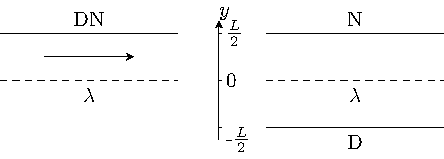
\includegraphics{fig_gnd_dn_lambda.pdf}
\caption{Partition function of Hamiltonian with DN and $\lambda$ boundary conditions. The width of the strip is $\pi$ due to folding. We unfold the cylinder and the new stripe have $N$ and $D$ boundary conditions on the left and right plus a $\lambda$ junction in the middle. }
\label{Fig in gnd_dn_lambda}
\end{figure}

In this appendix, we would like to calculate the amplitude for the setup shown in Fig.~\ref{Fig in gnd_dn_lambda}. In particular, the unfolded configuration has D/N boundary conditions at $x = \pm \frac{L}{2}$ and linking boundary condition at $x = 0$. The general solutions can be written as
\begin{equation}
\label{Normalized f in gnd_dn_lambda}
f(k, x) = 
\left\lbrace
\begin{aligned}
  A_1 e^{i kt} \cos(kx +\frac{1}{2}kL ) &  \quad x < 0  \\
  A_2 e^{ikt}  \sin(kx - \frac{1}{2}kL ) & \quad x > 0   \\
\end{aligned} \right. 
\end{equation}
As demonstrated in the {\bf\color{red}main text}, if we denote $f(k,x<0)\equiv\phi_1$ and $f(k,x>0)\equiv\phi_2$, the boundary condition at the junction reads
\begin{eqnarray}\begin{aligned}
\frac{\partial_x \phi_1}{ \partial_t \phi_1} = \lambda^2 \frac{\partial_x \phi_2}{ \partial_t \phi_2} = \tan^2 \theta\frac{\partial_x \phi_2}{ \partial_t \phi_2} \quad \theta \in [0,\frac{\pi}{2} ]  
\end{aligned}\end{eqnarray}
which implies
\begin{equation}
\label{Momentum in gnd_dn_lambda}
k = \frac{2\pi}{L}( n \pm \frac{\theta}{\pi} )  \quad n\in{\bf Z}
\end{equation}
It is evident that the momentum $k$ is shifted from integer multiple of $2\pi/L$ due to the $\lambda$ boundary condition in the middle. 
\begin{comment}
Thus, the normalized eigenfunctions are
\begin{equation}
f_n(x) = \sqrt{\frac{2}{L}}
\left\lbrace
\begin{aligned}
  \cos(kx +\frac{1}{2}kL ) &  \quad x < 0  \\
  \pm \sin(kx - \frac{1}{2}kL ) & \quad x > 0   \\
\end{aligned} \right. 
\qquad 
k = \frac{2\pi}{L}( n \pm  \frac{\theta}{\pi} )  \quad n \in \mathbb{Z} 
\end{equation}
Expand the field $\phi = \sum_n \phi_n f_n(x) $, the action and Hamiltonian becomes
\begin{equation}
  S = \frac{g}{2} \int dt \, \sum_{n \in \mathbb{Z} }\left(  \dot{\phi}^2_n + k^2 \phi_n^2 \right) \implies\quad   g \dot{\phi}_n  = \pi_n \quad \implies H =  
\frac{1}{2g}\sum_{n \in \mathbb{Z} } \pi_n^2 + ( kg )^2  \phi_n^2 
\end{equation}
\end{comment}

It is clear that the normalized eigenfunctions in Eq.~\eqref{Normalized f in gnd_dn_lambda} serves as orthonormal basis in mode expansion. Following the same procedure in \onlinecite{di_francesco_conformal_1997}, we have the Hamiltonian as
\begin{equation}
\label{H in gnd_dn_lambda}
H = \frac{1}{2} \sum_{n \in \mathbb{Z} } |k|  (a^{\dagger}_n a_n + \frac{1}{2} )
\end{equation}
where the momentum $k$ is defined in Eq.~\eqref{Momentum in gnd_dn_lambda}, and the creation and annihilation operators defined as usual
\begin{equation}
\begin{aligned}
a_n = \frac{1}{\sqrt{2}} ( \sqrt{ |k|g} \phi_n + \frac{i }{\sqrt{|k|g} }\pi_n  ) \\
a^{\dagger}_n = \frac{1}{\sqrt{2}} ( \sqrt{ |k|g} \phi_n - \frac{i }{\sqrt{|k|g} }\pi_n  ) \\
\end{aligned}
\end{equation}

The Casimir energy is the vacuum energy brought by the finite size of the setup. From Eq.~\eqref{H in gnd_dn_lambda} and define $x\equiv\theta/\pi$ in Eq.~\eqref{Momentum in gnd_dn_lambda}, we have
\begin{equation}
\begin{aligned}
E_c &= \frac{1}{4} \sum_{n \in \mathbb{Z}} | k| = \frac{\pi}{2L} ( \sum_{n \in \mathbb{Z}}  | n + x | + \sum_{n \in \mathbb{Z}}  | n - x |  ) \\  
&= \frac{\pi}{L} \Big[\sum_{n \ge 0 } ( n + x )^{-s} + \sum_{n \ge 0 }  ( n - x)^{-s}  +   x^{-s} \Big]\Big|_{s = -1} \\
&= \frac{\pi}{L} \left[ \zeta_{\rm H}( -1, x ) + \zeta_{\rm H}( -1, x ) +  x \right] \\
&= \frac{1}{2} ( - x^2 + x - \frac{1}{6})
\end{aligned}
\end{equation}
where we used the fact that the unfolded geometry has length $L=2\pi$. Thus the free energy reads
\begin{equation}
F = \beta E_c = - \frac{\beta}{2} B_2( x) 
\end{equation}
which agrees with the boundary state calculation in Eq.{\bf\color{red}where}



\section{$\lambda_1 \rightarrow \lambda_2$ Boundary State Amplitude}
\label{app:lambda_12}
% copy notes app. B

\begin{figure}[h]
\centering
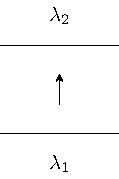
\includegraphics{fig_lambda_1_lambda_2.pdf}
\caption{Partition function between two boundary states of $S_i( \theta_1)$ and that of $S_j( \theta_2 )$}
\label{fig:fig_lambda_1_lambda_2}
\end{figure}

In this appendix, we calculate the amplitude between general boundary states defined in Eq.~\eqref{eq:Zab-bd}
\begin{equation}
\begin{aligned}
Z_{ab} &= \langle 0 | \exp\Big\{  \vec{b} R_b( \theta )    \vec{\bar{b}} \Big\}  \exp\Big\{ -\vec{b}^{\dagger}  (\mathbb{I}_2  \otimes M)  \vec{b} \Big\} \\
&\exp\Big\{  \vec{b}^{\dagger} R_a( \theta )    \vec{\bar{b}}^{\dagger} \Big\} | 0\rangle 
\end{aligned}
\end{equation}
where
\begin{equation}
\begin{aligned}
M &=  \frac{4\pi^2}{\beta} \text{diag}( 1, 2, \cdots ), \quad  \mathbb{I}_2 = \text{diag}( 1, 1) \\
R_i &= S_i( \theta ) \otimes \mathbb{I}
\end{aligned}
\end{equation}
Using the identity Eq.~\eqref{eq:second_id_in_app_pf_of_id} proven in App.~\ref{app:pf_of_id}, we have
\begin{equation}
Z_{ab} = \frac{1}{\det(1 - R_a^{\dagger} ( \mathbb{I}_2 \otimes M ) R_b )}
\end{equation}
From $|\det( R_a R_b^{\dagger})|  = 1$, free energy becomes
\begin{equation}
F = - \ln |Z_{ab}| = \ln |\det ( R_a R_b^{\dagger} - e^{- \mathbb{I}_2 \otimes M} )| .
\end{equation}
There are two cases to be considered, and we only take out the leading order term in $\beta$. 
\begin{itemize}
\item {\it case 1: }$S_1( \theta_1 ) \rightarrow S_2 ( \theta_2 ) $, the free energy is
\begin{equation}
\begin{aligned}
F & = \ln |\det ( R_1( \theta_1 )  R_2^{\dagger}( \theta_2 )  - e^{- \mathbb{I}_2 \otimes M} )| \\
  & = \ln \left| \det
\begin{bmatrix}
-\cos 2 \Delta \theta \mathbb{I} - e^{-M}   & -\sin 2 \Delta \theta \mathbb{I}\\
- \sin 2\Delta \theta \mathbb{I}  &   \cos 2 \Delta \theta \mathbb{I} - e^{-M} \\ 
\end{bmatrix} \right| \\
& = \sum_i \ln [ 1 -  e^{- 2 \lambda_i }  ] \\
& = \frac{\beta}{4\pi^2} \int_0^{\infty} dx \ln [ 1 - e^{-2x} ]  = - \frac{1}{48 }\beta .
\end{aligned}
\end{equation}
\item {\it case 2:} $S_i( \theta_1 ) \rightarrow S_i( \theta_2 )$, where $i = 1 $ or $ 2$, 
\begin{equation}
\begin{aligned}
F & = \ln \det 
\begin{bmatrix}
\cos 2 \Delta \theta \mathbb{I} - e^{-M}   & \sin 2 \Delta \theta \mathbb{I}\\
- \sin 2\Delta \theta \mathbb{I}  &   \cos 2 \Delta \theta \mathbb{I} - e^{-M} \\ 
\end{bmatrix} \\
& = \sum_i \ln [ 1 - 2 \cos 2 \Delta \theta e^{- \lambda_i } + e^{- 2 \lambda_i }  ] \\
& = \frac{\beta}{4\pi^2} \int_0^{\infty} dx \ln [ 1 - 2 \cos 2 \Delta \theta e^{-x} + e^{-2x} ] ,
\end{aligned}
\end{equation}
where $\Delta \theta = \theta_2 - \theta_1$. This integral is an even function of $\Delta \theta$ and the $\Delta \theta > 0$ case reduce to the polylog and Bernoulli polynomial
\begin{equation}
\begin{aligned}
  F &= \frac{\beta}{4\pi^2} \left[ - \text{Li}_2 ( e^{2i |\Delta \theta|} ) - \text{Li}_2 ( e^{- 2i |\Delta \theta|} ) \right] \\
  & = \frac{\beta}{4\pi^2}  \left[ - 2\pi^2 B_2 (|x|) \right] \\
  &= - \frac{\beta}{2} B_2( |x| )  = \frac{\beta}{2} (| x| - x^2 - \frac{1}{6} ),
\end{aligned}
\end{equation}
where $x = \frac{\Delta \theta}{ \pi}$. 
\end{itemize}




%%% Local Variables:
%%% TeX-master: "bCFT_paper"
%%% TeX-PDF-mode: t
%%% End:


\bibliographystyle{plain}
\bibliography{bCFT}

\end{document}

%%% Local Variables: 
%%% TeX-PDF-mode: t
%%% End: 
